
\documentclass{article}

\usepackage{amsmath}
\usepackage{amscd}
\usepackage[tableposition=top]{caption}
\usepackage{ifthen}
\usepackage[utf8]{inputenc}

\usepackage{Sweave}
\begin{document}

\title{Assignment 3}
\author{Christopher Peters}
\maketitle

{\bf Assignment 3: Exercise 1}\\

The file Bleed.txt, in RSplidaAlpha\textbackslash RSplida text data, contains
field failure data on failures in aircraft engine bleed systems (each air-
craft has one such system) from a fleet of 2256 military aircraft. Use
these data to compute the Kaplan-Meier product limit estimator out to
500 hours of operation. Set this up in a table and do the computation
without the aid of a computer, unless you do your own programming
(e.g., in R or an Excel spreadsheet). Show the table outlining the com-
putations as part of your solution. You can use available software (e.g.
JMP or RSPLIDA) to check your answers.\\


{\bf Answer:}




\begin{center}
\begin{Schunk}
\begin{Sinput}
> print(qplot(Hours, KM, data = bleed.data))
\end{Sinput}
\end{Schunk}
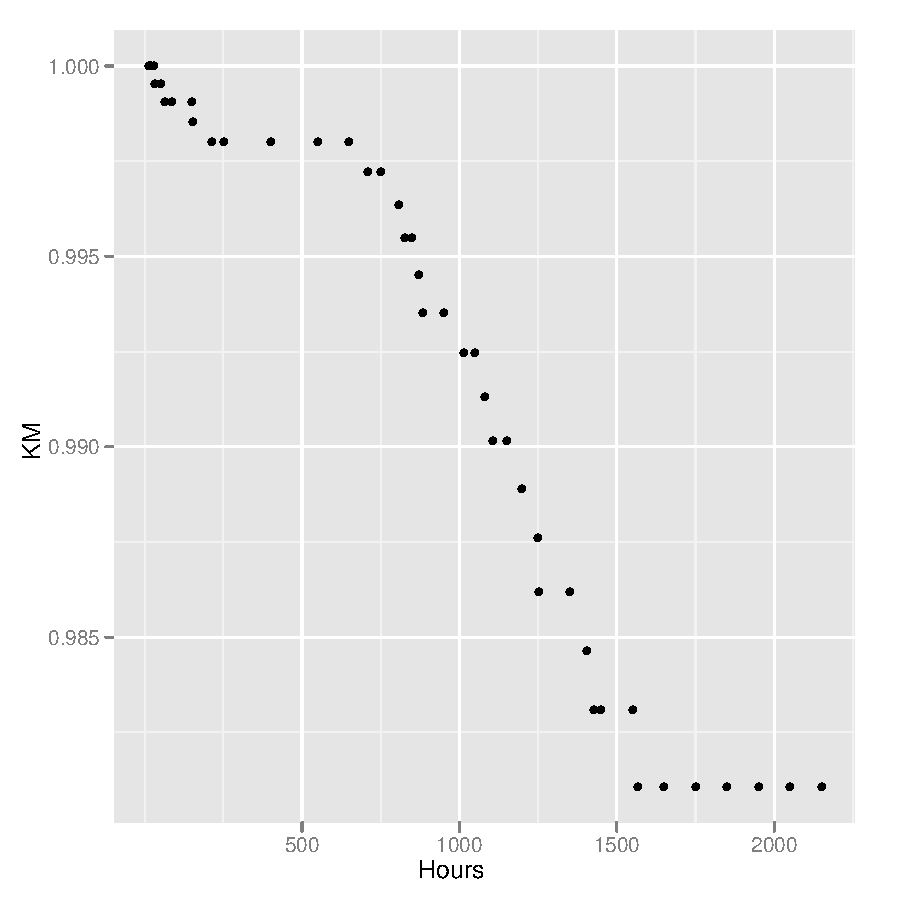
\includegraphics{assignment3_sweave-004}
\end{center}  

\end{document}
